\section{Выводы и результаты}
%%%%%%%%%%%%%%%%%%%%%%%%%%%%%%%%%%%%%
\subsection{Задача 1}
Было проведено тестирование работы метода сопряженных градиентов на матрицах Стильтеса с предобуславливанием на основе разложений $ILU(k)$, $MILU(k)$, $ILU(k, e)$. Тестирование проводилось на наборе из 80 разреженных матриц Стильтеса порядка 9.

Среднее число итераций метода сопряженных градиентов без предобуславливания на тестовом множестве – 95. Минимальное – 78, максимальное – 128.

На графиках приведены результаты тестирования для метода сопряженных градиентов с предобуславливанием.

Таким образом, качество предобуславливателя $ILU(k)$ растет с увеличением параметра $k$, но не имеет смысла брать параметр $k$ больше 2. Уже при $k=0$ метод сопряженных градиентов имеет значительно более высокую скорость сходимости.

$MILU(k)$ на тестовом множестве матриц показывает более высокую эффективность, и удовлетворительным является параметр $k=1$.
               
Предобуславливатель $ILU(0, e)$ на тестовых примерах незначительно отличался от предобуславливателя $ILU(0)$. Но видно, что не следует выбирать $e$ слишком большим: это ухудшит скорость сходимости.

\begin{figure}[ht]
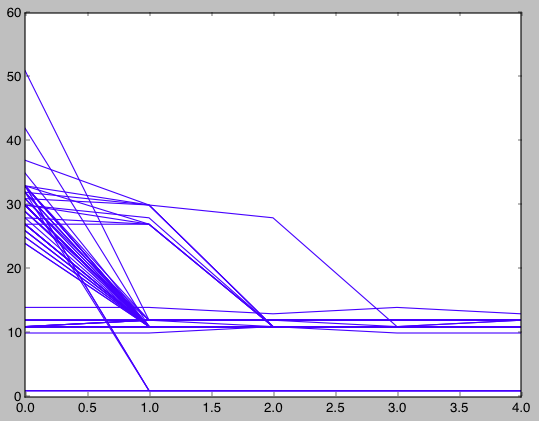
\includegraphics[width=\textwidth,keepaspectratio]{ilu_k}
\caption{Число итераций метода сопряженных градиентов с предобуславливанием $ILU(k)$ в зависимости от параметра $k$. Ось $Ox$ – параметр $k$, ось $Oy$ – число итераций.}
\end{figure}

\begin{figure}[ht]
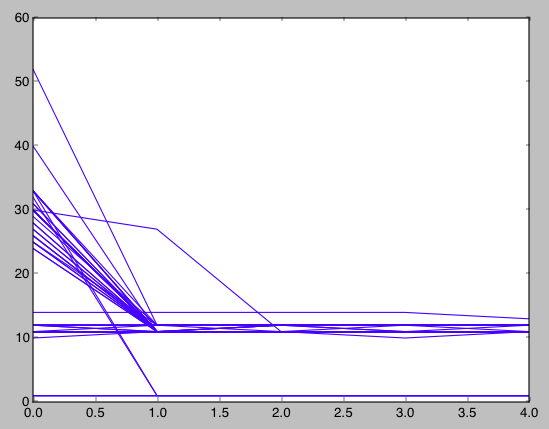
\includegraphics[width=\textwidth,height=\textheight,keepaspectratio]{milu_k}
\caption{Число итераций метода сопряженных градиентов с предобуславливанием $MILU(k)$ в зависимости от параметра $k$. Ось $Ox$ – параметр $k$, ось $Oy$ – число итераций.}
\end{figure}

\begin{figure}[ht]
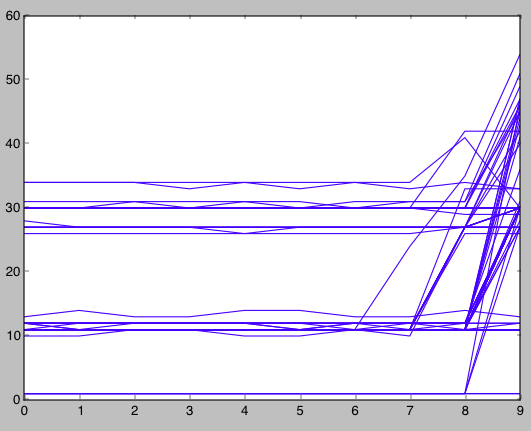
\includegraphics[width=\textwidth,height=\textheight,keepaspectratio]{ilu_0_e}
\caption{Число итераций метода сопряженных градиентов с предобуславливанием $ILU(0, e)$ в зависимости от параметра $e$. Ось $Ox$ – параметр $e$, масштаб: $10^{-8}$, ось $Oy$ – число итераций.}
\end{figure}





